\documentclass[a4paper,10pt]{report}
\usepackage[utf8]{inputenc}
\usepackage{fullpage}
\usepackage{amsmath}
\usepackage{amsfonts}
\usepackage{tikz}
\usepackage{graphicx}
\usepackage{mdframed}
\usepackage{color}
\usepackage{listing}
\usepackage{wrapfig}
\usepackage[parfill]{parskip}

% Title Page
\title{Facet-based Imaging}
\author{Benjamin Hugo}
\date{April 2014}

\begin{document}
\maketitle
\chapter{Introduction to Radio Astronomy}
In this section we give a very brief overview of what radio astronomy is, how the intensity of celestrial sources are quantified, how these intensity measurements are related to images (synthesis imaging),
the problems faced by large arrays taking measurements over large fields of view, and finally how they can be overcome. The focus of our work lies in acceleration of the synthesis imaging process, and in particular,
focussing on how the current memory intensive techniques required for wide-field imaging can be traded off at the expense of higher computation costs. This tradeoff is qualified by the recent shift towards using 
highly parallel platforms in all major computational fields; ranging in everything from computational chemestry, computing financial models of option pricing, through to radio astronomy. In particular we will be investigating 
the use of General Purpose Graphics Processing Units (GPGPU) in accelerating the facet-based convolutional gridding algorithm. More on this a bit later on.
\section{Brief history}
Through eons of visual observation mankind learned, amongst other things, the laws that govern the movement of the celestrial objects in the skies above him. In the last 500 years we've 
seen major advances in our ability to observe new phenomina, starting with the first optical telescope and manufacture of transparent glass. However these observations
were still restricted to the wavelengths of visible light. Radio waves are about one million times longer than light waves and often exposes areas of space opaque to visible light. The 
next series of improvements exploring this area came only by the 1930s when observations at longer wavelengths were made, after several failed attempts to receive radio emissions from the sun by the 
late nineteenth century. Herschel (1930) expanded the observable electromagnetic spectrum to the near infrared wavelengths: $0.35\mu m \leq\lambda\leq 1\mu m$. The most drastic change came when Jansky (1931) 
observed radiation from an extraterrestrial source (which wasn't the sun) with much longer wavelengths of $14.6m$ using a direction sensitive antenna array. By 1937 Grote Reber published the first observations 
in a professional astronomical journal. After World War II improved equipment and the use of the optical interferometer ultimately lead to the techniques of aperture synthesis still employed today. Ultimately all
historical development has been geared toward shorter wavelengths (see figure~\ref{fig_radio_window}), higher sensitivity, and higher angular resolution\cite{christiansenradiotelescopes,wilson2009tools}.

\begin{figure}[ht]
 \begin{mdframed}
 \centering
 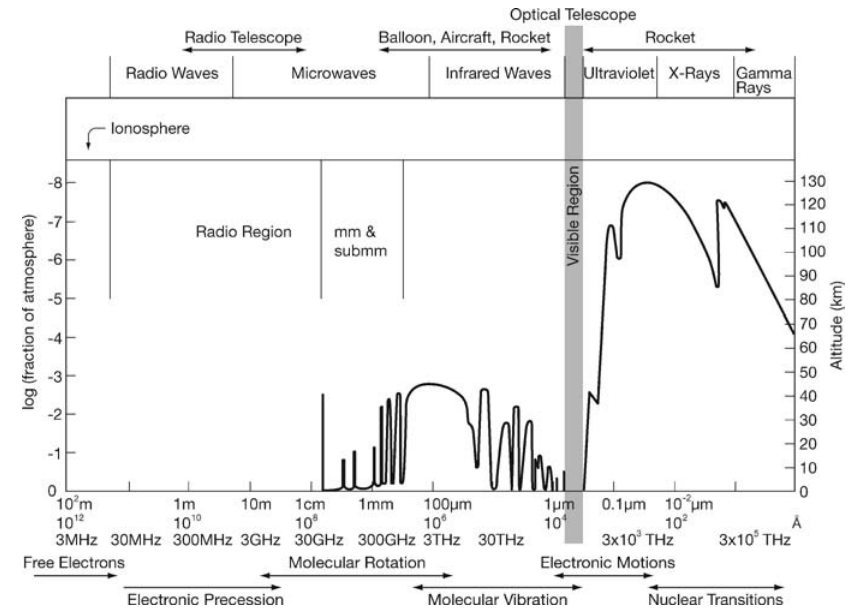
\includegraphics[width=0.8\textwidth]{images/radio_window.png}
 \caption[The radio window]{The radio window - Earth-based radio astronomy is bound to a range of wavelengths between $\lambda\approx 0.2mm$ and $\lambda\approx 20m$ by the molecular absorbtion bands of oxygen and water at the
 small wavelengths and the ionosphere at the long end. The figure shows at what altitude the incomming electromagnetic radiation is attenuated by a factor of 0.5 \cite{wilson2009tools}.}
 \end{mdframed}
 \label{fig_radio_window}
\end{figure}

\section{Measurement}
Some of the most important measurements of a celestrial object includes the object's angular size, position (according to some celestrial coordinate system) and the \textit{flux} density over a 
frequency spectrum of the object. The flux density is measured as the power per square meter per unit frequency, falling on a surface, normal to the direction of the source. This flux 
density of sources is often a very small value and the Jansky (abbreviated Jy) serves as the unit of measure \cite{christiansenradiotelescopes,wilson2009tools}:

\begin{equation*}
 1 Jy := 10^{-26}Wm^{-2}Hz^{-1}
\end{equation*}

Electromagnetic radiation is a wave phenominon stemming from both thermal and non-thermal sources propagating outward at the speed of light. Generally thermal sources follows Rayleigh's approximation to the radiation 
law and states that a black-body will have a flux density $S\propto \upsilon^2T$ where the black-body radiates at a temperature $T^oK$. The spectra of planets and stars are of this type. On the other hand in non-thermal 
sources, one of the most common generators of electromagnetic ratiation magnetic is \textit{synchrotron emission}. This process accelerates the electrons passing through electric fields. A significant portion of radio 
astronomy focusses on the non-thermal sources. These are generally very intense sources of electromagnetic radiation and are very far away \cite{christiansenradiotelescopes}.

It is worth noting that not only are radio telescopes used to observe continuous spectra consisting of a wide band of frequencies, but it is also critical sometimes to isolate a number of
spectral lines for observation. These don't originate from large black-body structures, but focusses on the detection of certain molecules, such as neutral hydrogen (at $\lambda = 21 cm$),
hydroxyl ($\lambda \approx 21 cm)$. These spectral lines are vital in measuring radial velocities through Doppler frequency shift \cite{christiansenradiotelescopes}.

The wave fronts from these sources can be viewed as planar fronts if the source of the radiation is sufficiently far away. This is not 
necessarily true for sources within our own galaxy for example. Furthermore if the wavelength is much smaller than the scale of the observing antenna the radiation can be 
viewed as traveling as rays. The total flux of a source is then obtained over the solid angle subtended by the source (see figure~\ref{fig_measuring_source_brightness}) as 
follows \cite{wilson2009tools}:

  \begin{equation}
    S_v := \int_{\Omega_s}{I_v(\theta,\phi)\cos{\theta}d\Omega}
  \end{equation}
  and the infinitesimal power intercepted by an infinitesimal surface is:
  \begin{equation}
    dP = I_v\cos{\theta}d\Omega\ d\sigma d\upsilon
  \end{equation}

  where:\\
  $dP = $ infinitesimal power (in watts)\\
  $d\sigma = $ infintesimal area of surface\\
  $d\upsilon = $ infintesimal bandwidth\\
  $\theta = $ angle between the direction to $d\Omega$ and normal to the surface\\
  $I_{v} =$ specific intensity in $Wm^{-2}Hz^{-1}sr^{-1}$ where r is the distance between the source and antenna.\\
  
\begin{figure}[ht]
\begin{mdframed}
 \centering
 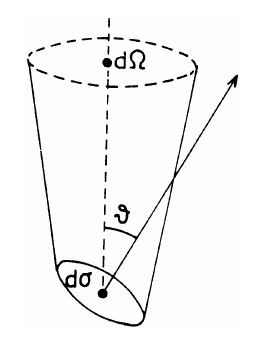
\includegraphics[width=0.2\textwidth]{images/measuring_source_brightness.png}
 \caption[Source brightness]{Flux density over a small area per unit frequency \cite{wilson2009tools}.}
\end{mdframed}
 \label{fig_measuring_source_brightness}
\end{figure}

It should be clear that since most sources are extremely faint, the telescopes needed to detect them will be some of the most sensitive instruments ever designed. Although we cannot
cover antenna theory extensively here, it is essential to briefly relate how the electromagnetic radiation covered earlier, is measured by instrumentation in general.

\bibliography{bibfile}
\bibliographystyle{plain}
\end{document}          
